
\documentclass[letterpaper,12pt]{article}
\usepackage{tabularx} % extra features for tabular environment
\usepackage{amsmath}  % improve math presentation
\usepackage{float}
\usepackage{pdfpages}

\usepackage{multicol}
\usepackage{graphicx} % takes care of graphic including machinery
\graphicspath{ {./figures/} }
%\usepackage[margin=1in,letterpaper]{geometry} % decreases margins
%\usepackage{cite} % takes care of citations
\usepackage[final]{hyperref} % adds hyper links inside the generated pdf file
\hypersetup{
	colorlinks=true,       % false: boxed links; true: colored links
	linkcolor=blue,        % color of internal links
	citecolor=blue,        % color of links to bibliography
	filecolor=magenta,     % color of file links
	urlcolor =blue         
}
\usepackage[margin = 1in,headsep=0.5cm,headheight=2cm,letterpaper]{geometry} 

\usepackage{fancyhdr}
\pagestyle{fancy}
%\cfoot{center of the footer!}
\renewcommand{\headrulewidth}{0.1pt}



\begin{document}
\thispagestyle{empty}

\title{Fall 2022 EE301  \protect\\ Homework 1}
\author{Ahmet Akman 2442366 \protect\\ Hasan Oğuzhan Gök 2443083 }
\date{\today}
\maketitle
\tableofcontents
%\begin{abstract}
%abstract
%\end{abstract}
\section{Question 1 Solution}
Input/output relation: \(y_1(t)= x(t)cos(2 \pi f_0 t) \)
\\ Properties:

\begin{itemize}
    \item \textbf{Memory:} The system is memoryless since the output is only depend on the current t value.
    \item \textbf{Linearity:} The system is linear it can be shown as follows: \begin{equation}\begin{split}
        \underline{input} &\Rightarrow \underline{output} \\
        x_1(t)  & \Rightarrow x_1(t) cos(2\pi f_0 t) \\
        a x_2(t) & \Rightarrow  a x_2(t) cos(2\pi f_0 t) \\
        x_1(t) +  a x_2(t)  &\Rightarrow x_1(t) cos(2\pi f_0 t) + a x_2(t) cos(2\pi f_0 t)      \end{split}
    \end{equation} 
    So the linearity holds.
    \item \textbf{Causality:} Since the system is memoryless it can be said that the system is causal.
    \item \textbf{Time-Invariance:} The system is time-varying since a time shift in the input does not result in same time shift in the output. \begin{equation}
        \begin{split}
            Let x_2(t) &= x_1(t-t_0) \\
            y_1(t) &= x_1(t) cos(2 \pi f_0 t) \\ 
            y_2(t) &= x_2(t) cos(2 \pi f_0 t)\\
            y_1(t-t_0) &=    x_1(t-t_0) cos(2 \pi f_0 (t-t_0))\\
            \text{However  } y_2(t) & \neq y_1(t-t_0)
        \end{split}
    \end{equation}
    \item \textbf{Stability:} Since \(-1 \leq cos(alpha) \leq 1\) if the x(t) is bounded the y(t) is bounded as well. So the system is stable.
\end{itemize}
Input/output relation: \(y_2(t)= c_1 x(t) + c_2 x^2(t) \)
\\ Properties:
\begin{itemize}
    \item \textbf{Memory:} The system is memoryless since the output is only depend on the current t value.
    \item \textbf{Linearity:}The system is non-linear and it can be shown as follows: \begin{equation}\begin{split}
        \underline{input} &\Rightarrow \underline{output} \\
        x_1(t)  & \Rightarrow c_1 x_1(t) + c_2 x_1^2(t) \\
        a x_2(t) & \Rightarrow  c_1 a x_2(t) + a^2 c_2 x_2^2(t) \\
        x_1(t) +  a x_2(t)  & \not\Rightarrow   c_1 (x_1(t) + a x_2(t)) + c_2 (x_1^2(t) + a^2 x_2^2(t) )
          \end{split}
    \end{equation} 
    \item \textbf{Causality:} Since the system is memoryless it can be said that the system is causal.
    \item \textbf{Time-Invariance:} The system is time invariant and it can be shown as follows;
    \item \begin{equation}
        \begin{split}
            \text{Let } x_2(t) &= x_1(t-t_0) \\
            y_1(t) &= c_1 x_1(t) + c_2 x_1^2(t) \\ 
            y_2(t) &= x_2(t) + c_2 x_2^2(t) \\
            y_1(t-t_0) &=    c_1 x_1(t-t_0) + c_2 x_1^2(t-t_0) \\
            \text{Then  } y_2(t) &= y_1(t-t_0)
        \end{split}
    \end{equation}
    \item \textbf{Stability:} System is stable, that is if the input of \(x(t)\) is bounded output is also bounded.
\end{itemize}


Input/output relation: \(y_3(t)= x(t)+4 \)
\\ Properties:
\begin{itemize}
    \item \textbf{Memory:} The system is memoryless since it just shifts the input signal.
    \item \textbf{Linearity:} Let  \(x(t)\) be equal to 0. The output is not equal to the 0. So the system is not linear.
    \item \textbf{Causality:} Since the system is memoryless it is causal.
    \item \textbf{Time-Invariance:} Any time shift on the input signal results in same amount of time shift on the output signal. So the system is time invariant.
    \item \textbf{Stability:} The system is stable, as the output is just the time shifted version of the input. 
\end{itemize}

Input/output relation: \(y_4(t)= x(t/3) \)
\\ Properties:
\begin{itemize}
    \item \textbf{Memory:}  The system is with memory since it squeezes the input signal.
    \item \textbf{Linearity:} The system is linear.
    \item \textbf{Causality:} Since the output may depend on different time instant other than the current t the system is not causal.
    \item \textbf{Time-Invariance:} As the input signal is squeezed the time shift in the input may not result in same amount of shift in the output.
    \item \textbf{Stability:} The system is stable as the magnitude stays for this system always.
\end{itemize}

Input/output relation: \(y_5(t)= t x(t+5) \)
\\ Properties:


\begin{itemize}
    \item \textbf{Memory:} The system is with memory because of the t+5 term.
    \item \textbf{Linearity:} The system is linear because the result stays linear if we multiply the input with a constant and sum it with another input. 
    \item \textbf{Causality:} The system is not causal because of the fact that the value of the input at t+5 time instant is used.
    \item \textbf{Time-Invariance:} The system is time-varying. The reason can be expressed as follows: \begin{equation}
        \begin{split}
             x_2(t+5) &= x_1(t+t_0+5) \\
             y_2(t) &\neq y_1(t) 
        \end{split}
    \end{equation}
    \item \textbf{Stability:} System is not stable consider the case where time is at infinity.
\end{itemize}

Input/output relation: \(y_6(t)= u(x(t)) \)
\\ Properties:
\begin{itemize}
    \item \textbf{Memory:} System is memoryless since the output depend only on the current input.
    \item \textbf{Linearity:} The system is not linear. Consider the case \(t = 0^- \and t = 0^+\)
    \item \textbf{Causality:} Memoylessness implies the system is causal.
    \item \textbf{Time-Invariance:} The system is time invariant. The shift in input leads same amount of shift in output.
    \item \textbf{Stability:} The system is stable. The outputs are bounded as long as inputs are bounded.
\end{itemize}



\section{Question 2 Solution}
\subsection{a)}
To be able to find the output signals the input signals are convolved with the inputs. The outputs are obtained with the computations given below;
\begin{equation}
    \begin{split}
        h(t) \ast 1 = \int_{-\infty}^{\infty} \alpha^{\tau-t} u(\tau-t)  \,d\tau  
    \end{split}
\end{equation}
\subsection{b)}
\section{Question 3 Solution}
LTI systems are characterized by ther impulse response. Therefore the output can be written as \(y[n] = x[n] - x[n-1]\).


\subsection{a)}
This system is very similar to derivate operation in calculus which can be expressed as    \(\lim_{\Delta t \to 0} y(t+ \Delta t) = \frac{x(t+ \Delta t) - x(t)}{\Delta t}\).
  Moreover, it operates same as derivative in terms of detecting the edges. Therefore this equation in discrete domain familiar to derivative operation in calculus since both calculates the changes in function in a small interval and edge points.
\subsection{b)}
Since the system is LTI, output to arbitrary input can be calculated by convolving the input with the impulse response.This can be expressed as: \newline
 \[y[n]= x[n] * h[n] = x[n]* \delta [n] - x[n] * \delta [n-1]= x[n]- x[n-1]\]
\subsection{c)}
For c the output is \( y[n]= e^{j \Omega_0 n} (1-e^{-j \Omega_0 n})\).\newline
To calculate $|y[n]|$ we tried to express the output in the form of :
\[y[n]=C[cos(\Omega_0 n) + jcos(\Omega_0 n)]\] where we can conclude that the magnitude of output is some C. To do that we multiplied and divided the output y[n] with \(e^{j \Omega_0 n/2}\).
As a result we obtained:
 \[y[n]=\frac{e^{j (\Omega_0 n+1/2)}-e^{j (\Omega_0 n-1/2)}}{e^{j (\Omega_0 n/2}}\].

 Then this equation equals to : \(y[n]= e^{j \Omega_0 (n-1/2)}(e^{j \Omega_0 n/2}-e^{-j \Omega_0 n/2})\)

 Using complex definitons of sine and cosine this equation yields to: \[y[n]= 2sin(\Omega_0 /2)[jcos(\Omega_0 (n-1/2))+sin(\Omega_0 (n-1/2))]\]

 Thus we can conclude that $|y[n]|= 2sin(\Omega_0 /2)$

\subsection{d)}

For \begin{equation}
    \begin{split}
        \Omega_0 = 0 \quad |y[n]|&= 2sin(\Omega_0 /2)=0\\
 \Omega_0 = \frac{2\pi}{8} \quad |y[n]|&= 2sin(\Omega_0 /8)=0.765\\
 \Omega_0 = \frac{2\pi}{4} \quad |y[n]|&= 2sin(\Omega_0 /4)=1.41\\
 \Omega_0 = \frac{2\pi}{2} \quad |y[n]|&= 2sin(\Omega_0 /2)=2
    \end{split}
\end{equation}
This system is similar to derivativ operation. As explained in part a this outputs tell us the change in function. We can conclude that for \( \Omega_0 = 0\) the function does not change.In calculus derivate is 0. In addition for  \( \Omega_0 = \pi \) the function changes faster.
\subsection{e)}

\subsection{f)}
Since these operation is similar to derivation it can be used to find the changes in function.In other words it may help us to detect edges in our signal. We can see from part e and part d that magnitude of function increases as the change in function increase.In addition, the point may get closer to the edges.
\section{Question 4 Solution}
\subsection{a)}
\subsection{b)}
\subsection{c)}

\subsubsection{i)}

\subsubsection{ii)}
\section{Question 5 Solution}
\subsection{a)}
In part 5, we convolved the input signal \(x[n] = sin(\frac{2\pi n}{7} )\) and impulse response \(h[n] = u[n] - u[n-L]\) to find output signal \(y[n]\) in MATLAB.
\subsubsection{i)}
In this part N(signal length) was equal to 20. Then following signal was plotted.
\begin{figure}[H]
    \centering
    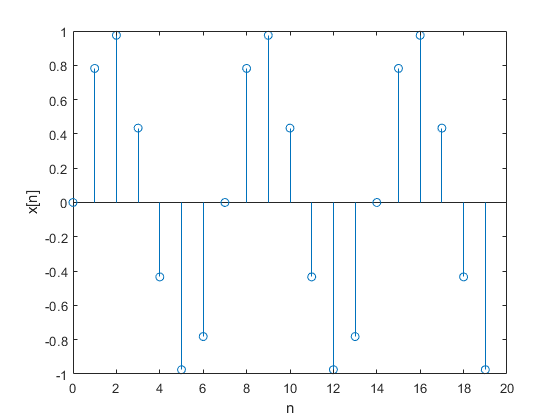
\includegraphics[width = 0.75\textwidth]{i.png}
    \caption{Signal x[n]}
    \end{figure} 
    
\subsubsection{ii)}
Impulse response \(h[n]\) was created with amplitude 1 and pulse duration L. L was equal to 14 in this example.
\begin{figure}[H]
    \centering
    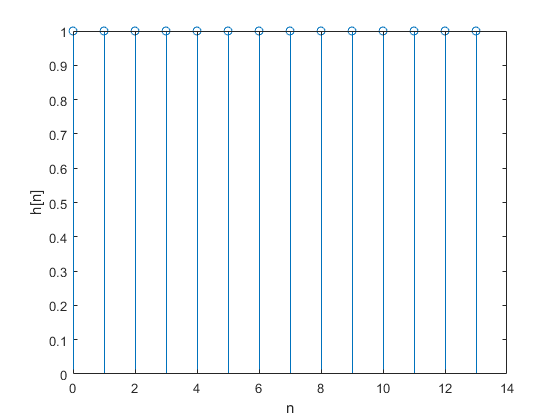
\includegraphics[width = 0.75\textwidth]{i2.png}
    \caption{Impulse Response}
    \end{figure} 
    
\subsubsection{iii)}
In this part we implemented convolution operation. Since our signals are not infinity we used zero padding to be able to compute convolution. Then we obtained \(y[n]\) using for loop. Since zero padding leads to mistake on last a few values, we only plotted correct ones. Following plot shows the output of convolution operation with padding.
\begin{figure}[H]
    \centering
    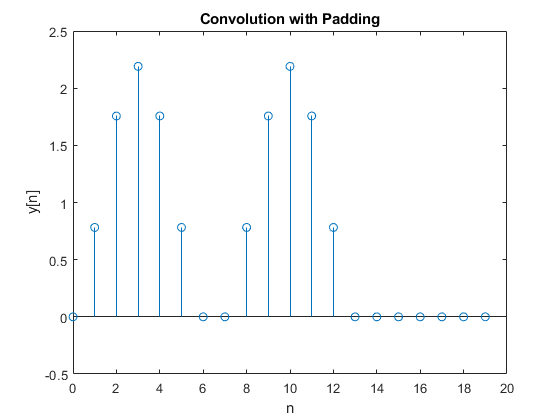
\includegraphics[width = 0.75\textwidth]{convwithpadding.png}
    \caption{Convolution with Padding}
    \end{figure} 
    
\subsubsection{iv)}
Convolution operation executed in last part can be done by conv method in MATLAB. Following graph shows the convolution results. 
\begin{figure}[H]
    \centering
    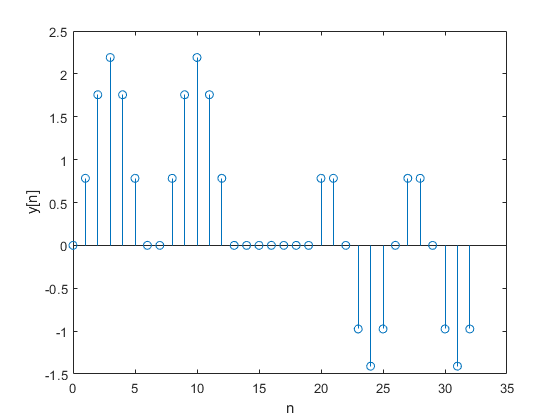
\includegraphics[width = 0.75\textwidth]{i4.png}
    \caption{Convolution Operation Using conv Method}
    \end{figure} 
    As indicated in figures in section iii and iv , the convolution method in MATLAB results in more acquarete results. Due to the zero padding method in part iii, results after n>N are nor correct.


\subsection{b)}
To observe pulse duration length(L) effect on output signal, random signal input convolved with \(h[n]\) by changing L in the \(h[n] = u[n] - u[n-L]\). L was chossen to be 2 , 15 and 25.
Following graph shows the random signal \(x[n]\).
\begin{figure}[H]
    \centering
    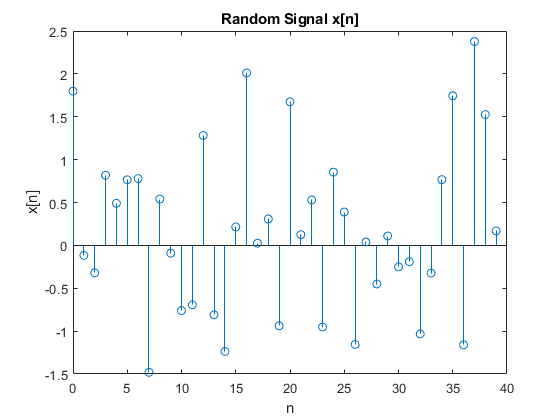
\includegraphics[width = 0.75\textwidth]{b_signal.png}
    \caption{Random Signal}
    \end{figure} 


The convolution result \(y[n] = x[n] * h[n]\) with L = 2 is shown in following figure.
\begin{figure}[H]
    \centering
    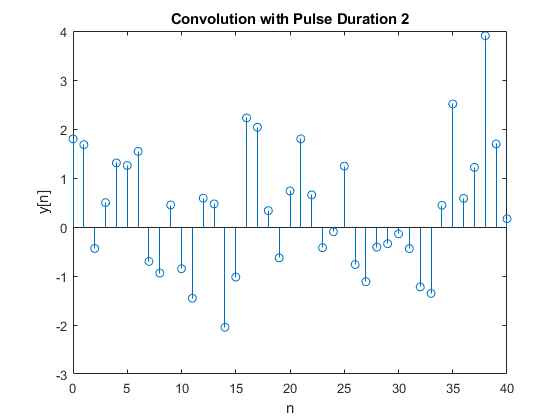
\includegraphics[width = 0.75\textwidth]{b_duration2.png}
    \caption{Convolution Result with L=2}
    \end{figure} 


    The convolution result \(y[n] = x[n] * h[n]\) with L = 15 is shown in following figure.
    \begin{figure}[H]
        \centering
        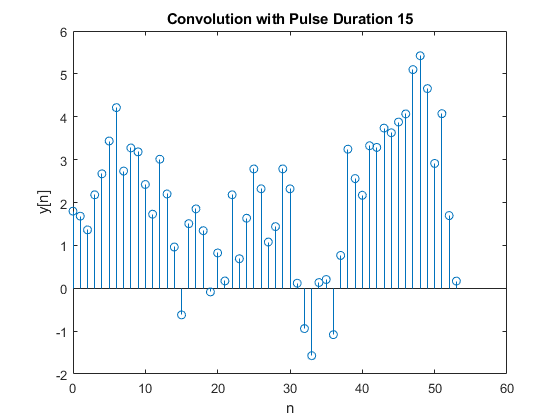
\includegraphics[width = 0.75\textwidth]{b_duration15.png}
        \caption{Convolution Result with L=15}
        \end{figure} 

        
        The convolution result \(y[n] = x[n] * h[n]\) with L = 25 is shown in following figure. 
        \begin{figure}[H]
            \centering
            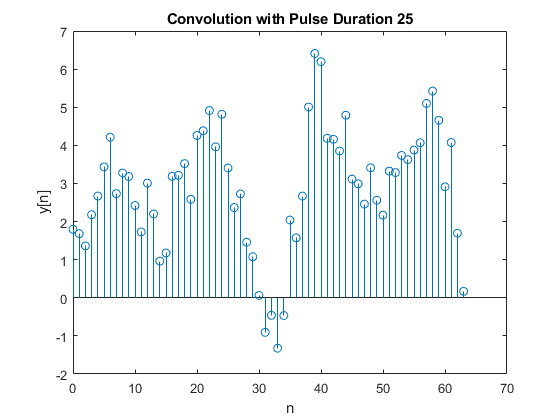
\includegraphics[width = 0.75\textwidth]{b_duration25.png}
            \caption{Convolution Result with L=25}
            \end{figure} 



As shown in al figures, the smoothness of graph increases as L increases. Although it gets smoother, these systems called "averaging filter" ,may lead to some loses. This filter can be used to observe a signal's trend and obtain meaningfull data.




\end{document}

%%%%%%%%%%%%%%%%%%%%%%   EXAMPLE TABLE   %%%%%%%%%%%%%%%%%%%%%%%%%%%%%%%%
\begin{table}[H]
\begin{center}
    \caption{Resistance reading by color code convention.}
    \vspace{2mm}
    \begin{tabular}{||c | c | c||} 
        \hline
        Color Order & Value & Tolerance \\ [0.5ex] 
        \hline\hline
        Brown / Black / Red / Gold & 1k\( \Omega \) & \( \% \) 5  \\ 
        \hline
        Yellow / Violet / Red / Gold & 4.7k\( \Omega \) & \( \% \) 5   \\
        \hline
        Brown / Grey / Orange / Gold & 18k\( \Omega \) & \( \% \) 5  \\ [1ex] 
        \hline
    \end{tabular}
\end{center}
\end{table}


%%%%%%%%%%%%%%%%%%%%%%   EXAMPLE IMAGE   %%%%%%%%%%%%%%%%%%%%%%%%%%%%%%%%
\begin{figure}[H]
\centering
\includegraphics[width = 0.75\textwidth]{5.png}
\caption{Circuit schematic for the step 5}
\end{figure} 

%%%%%%%%%%%%%%%%%%%%%%   EXAMPLE IMAGE FROM PDF   %%%%%%%%%%%%%%%%%%%%%%%%%%%%%%%%
\begin{figure}[H] \centering{
	\includegraphics[scale=0.25]{2a_plot.pdf}}
	\caption{Experiment 2}
\end{figure}
